
\chapter{粒子模拟程序用户界面}

为了提高模拟程序的易用性,我们基于Impact\cite{PIC_ji2000}开发了图形化的用户界面(GUI)。
GUI使用python内置的tkinter模块进行开发,并依赖matplotlib, numpy, scipy 三个库。
GUI可以跨平台使用,我们在Windows, Linux, MacOS均进行了测试。
GUI主要分为主界面,预处理,后处理三部分。用户可在github上自由下载本界面:

\begin{center}
  \href{https://github.com/zhicongliu/ImpactGUI.git}{https://github.com/zhicongliu/ImpactGUI.git}
\end{center}

GUI主界面如图\ref{fig:ImpactGUI}所示,菜单栏包括“存档”、“读取”、“切换内核”、以及“帮助”等功能。
用户可以在主界面内设置Impact 运行所需要的参数,比如初始时间步长,步数,束流能量,流强,空间电荷网格数,粒子分布,Lattice结构等。
除此之外,用户还可以通过高级设置(Advanced Setting)对输入参数进行更加详细的设置。
在用户输入相应的参数后,点击运行(Run)按钮,GUI会自动调取Impact内核,使用所给定参数进行模拟。
GUI还包括数据预处理(Pre-Process)和后处理(Post-Process),
预处理主要用于计算腔体的同步相位。GUI后处理主要用于数据可视化,根据Impact内核产生的输出文件作图。

\begin{figure}
  \centering
  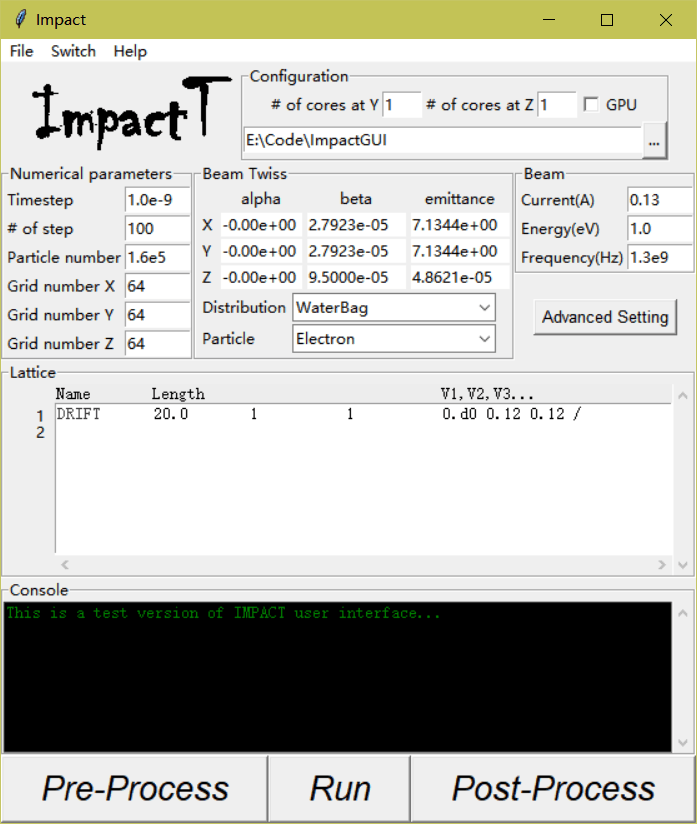
\includegraphics[width=0.8\textwidth]{ImpactGUI.png}
  \caption{Impact用户界面}\label{fig:ImpactGUI}
\end{figure}

